\section{Introduction}

Pacemakers are safety-critical \acp{CPS} that control the pacing of a
heart for providing therapy for bradycardia -- abnormally slow pacing of
the heart. %Such devices must operate in a fail-safe manner all the
%time. 
Between 1990-2000, close to 200,000 pacemakers have been
recalled due to software related
failures~\cite{alemzadeh13}. Considering this, there is a need for the
development of better processes for validation and certification of such
devices. We propose the well known, engineering
technique of \emph{emulation}~\cite{patel2015survey} to tackle this
problem. Emulation, also known as hardware-in-the-loop simulation, is
used to validate controllers (such as motor controllers) by running them
in closed-loop with the actual plant (e.g., the synchronous motor).
However, for emulation of pacemakers, the use of the actual plant
(i.e. animal / human organs) is limiting. Hence, there is a need for the
development of high-fidelity heart models that can provide the required
real-time response to facilitate emulation. Bioengineering heart
models~\cite{Trayanova2014} provide excellent model fidelity at the
expense of computation time as the simulation of a single heart beat may
take several hours making them not suitable for emulation.

Recently, timed automata~\cite{zhihao12} based heart models have been
developed primarily for model checking. These models abstract the
continuous dynamics and hence, are unsuitable for emulation. In contrast
to this, \acf{HIOA}~\cite{alur2015book, raskin05} is used for modelling
the forward conduction system of the heart using 33 nodes
in~\cite{chen14}.
This work is the starting point for real-time
emulation by demonstrating that \simulink can be used for closed-loop
verification of pacemakers. However, this work has limited model
fidelity and the limitations of the tool \simulink are inherited by the
developed approach. \simulink has semantic limitations, as the semantics
of composition is unclear. Moreover, there is no
direct correspondence between the \simulink model and the \ac{HIOA}
models. Finally, \simulink generated code has scalability issues when 
generating large networks, as we will show.

% We develop an approach by combining node models (which are extensions
% to the models developed by~\cite{chen14}) with \emph{path models} (in
% timed automata) to accurately model the conduction delay between
% nodes. We are, thus, able to model the re-entrant behaviour of the
% heart.

 For modular code generation, we
have developed an approach based on the well known synchronous
languages~\cite{benveniste03}. % We formalise a subset of \ac{HIOA} called
% Synchronous Hybrid Input Output Automata \ac{SHIOA}.
Using the concept of delayed synchronous composition~\cite{SlLanguage},
we are then able to produce modular code for each node separately. The
generated code is both smaller and has faster execution times. In addition,
the generated code accurately captures the specification in \ac{HIOA},
similar in spirit to Ptolemy~\cite{ptolemaeus2014system} and
Z\'{e}lus~\cite{bourke13zelus}. However, unlike these approaches, the
presented approach does not depend upon dynamic numerical solvers, which
are not ideal for the \textit{emulation} of the heart.

\ignore{One reason that these malfunctions arise is due to the lack of
  proper validation. Unlike the ideas of hardware-in-the-loop testing,
  also known as \emph {emulation}~\cite{patel2015survey}, it is not
  possible to test on an actual heart. Further, unlike the hardware
  which is almost identical during mass production, each individual
  heart is different. Thus there is a need to develop a virtual heart
  that is tailored to an individual person and achieve personalised
  healthcare~\cite{Trayanova2014}. This idea can be extended to a
  network of human organs, resulting in a virtual human.

  Typically these biological models are developed by biomedical
  engineers. They mimic the heart's working at the molecular
  level~\cite{Trayanova2014}. To simulate one heart beat takes several
  hours, if not days. These models are very computationally intensive
  and are not suitable for real-time emulation, which is required for
  closed-loop testing of time-critical controllers such as cardiac
  pacemakers. Further, the models are very complex and hence are not
  amenable for formal verification. Thus, there is a need to develop
  abstract models by computer systems engineers that (1) \emph{capture
    the behaviour} of the heart (plant) from a pacemaker's
  (controller's) point of view, (2) \emph{allows for real-time
    emulation} of the heart such that it is possible for closed-loop
  simulation and (3) \emph{are amenable for formal verification} of
  functional and timing properties.

  The continuous dynamics of a plant (e.g. heart) and the discrete
  behaviour of a controller (e.g. pacemaker) result in so called hybrid
  systems. These are often formally described using
  \acf{HIOA}~\cite{alur2015principles,raskin05,chen201487}. However,
  these are non-deterministic and are problematic for generating
  constructive models. A more abstract deterministic model will enable
  us to develop constructive/synthesizable models~\cite{Lee2014}. Also,
  it is easier to draw trusted conclusions from simulations of
  deterministic models. Based on the well-known synchronous
  approach~\cite{benveniste03}, we present a deterministic semantics for
  \ac{HIOA} and show constructive models in this paper.

  Traditional \ac{CPS} design uses commercial tools such as \simulink
  for plant simulation and emulation. However, such designs do not
  preserve formal semantics of the models and are more verbose to
  describe. Academic tools for code generation from \ac{HIOA} models
  such as Ptolemy~\cite{ptolemaeus2014system} and
  Z\'{e}lus~\cite{bourke13zelus}. While these tools preserve the formal
  semantics, their reliance on dynamic numerical solvers makes them
  unsuitable for real-time emulation of plants. Such tools are capable
  of expressing the full non-deterministic nature of \acp{HIOA} rather
  than the deterministic subset described here.}

An overview of the proposed modular compilation approach is presented in
Figure~\ref{fig:overview}. It has two steps: (1) given a network of
\acp{HIOA}, step 1 generates a semantic preserving \ac{FSM}
representation of each \ac{HIOA} in the network. (2) Given a network of
such \acp{FSM}, step 2 then composes them using the synchronous parallel
operator ($||$) enabling generation of efficient `C'-code. Step 1 is
presented in Section~\ref{sec:codeGen}. Step 2 is presented in
Section~\ref{sec:composition}.


\begin{figure}[bthp]
  \centering \scalebox{0.7}{ % Define block styles
\tikzstyle{fileS} = [rectangle, draw, fill=red!20, 
text width=4em, text centered, minimum height=3em]
\tikzstyle{process} = [rectangle, draw, fill=blue!15, 
text width=9em, text centered, rounded corners, minimum height=4em]
\tikzstyle{line} = [draw, -latex', ultra thick]


\begin{tikzpicture}
% Place nodes

%-----------------------------------------------------------------------
\node [fileS,fill=red!10] (HA1) {$HIOA_1$ ($Def.~\ref{def:ha}$)};
\node[right of = HA1, node distance = 1.3cm](PAR){\Large $\dots$};
\node [fileS,,fill=red!10,right of = PAR, node distance = 1.3cm] (HA2) 
	{$HIOA_2$ ($Def.~\ref{def:ha}$)};	
%\node[below of = PAR, node distance=1.3cm, text width=3.7cm, text centered]
%	(TNHA){Network of HA};
%\node[draw, thick, inner sep=0.3cm, fit=(HA1) (HA2)] (NHA) {};

\node[draw, dashed, inner sep=0.3cm,
	label={[label distance=0cm]90:Section~\ref{sec:HA}}, 
	fit= (HA1) (HA2)] (S1) {};
%-----------------------------------------------------------------------


%\node [process, below  of = PAR, node distance = 2.2cm] (GSHA) {Generate FSM (step~1, Sec~\ref{sec:shaGeneration})};

%-----------------------------------------------------------------------
\node [fileS, below of = HA1, fill=red!20, node distance = 3.3cm] 
(FSM1) {$FSM_1$ ($Def.~\ref{def:ha}$)};
\node[right of = FSM1, node distance = 1.3cm](PAR){\Large $\dots$};
\node [fileS,,fill=red!20,right of = PAR, node distance = 1.3cm] (FSM2) 
{$FSM_2$ ($Def.~\ref{def:ha}$)};	

\node[draw, dashed, inner sep=0.3cm,
label={[label distance=0cm]90:Section~\ref{sec:codeGen}}, 
fit= (FSM1) (FSM2)] (S2) {};

%-----------------------------------------------------------------------
\node [fileS,,fill=blue!20, text width=8em, below of = PAR, node distance = 3.3cm] (PC) 
{$FSM_1 || FSM_2$ };
\node[ dashed, inner sep=0.1cm,
label={[label distance=0cm]90:Section~\ref{sec:composition}}, 
fit= (PC)] (S3) {};


%\node[draw, dashed, inner sep=0.2cm,
%	label={[label distance=0cm]60:Section~\ref{sec:SHA}}, 
%	fit= (GFSM)(CC)] (S3) {};

%--------------------------------------------------------------------------------
%edges
\draw [line] (HA1.south) -- (FSM1) node[midway, left]
{Step~1:  Code generation};
\draw [line] (HA2.south) -- (FSM2);
\draw [line] (FSM1) -- (FSM1|-PC.north) node[midway, left]
{Step~2:  Parallel composition};
\draw [line] (FSM2) -- (FSM2|-PC.north);
%\draw [line] (NSHA) -- (NSHA-|GFSM.west);
%\draw [line] (GFSM) -- (GFSM|-CC.south);

\end{tikzpicture}     }
  \caption{Overview of the proposed modular code generation
    approach \label{fig:overview}}
\end{figure}

\begin{figure*}[hbpt]
  \centering {
	\centering
	\subfigure[\label{fig:heart} Diagram of the heart. Reproduced 
	from~\cite{zhihao12}]{
       \framebox[0.31\textwidth]{
				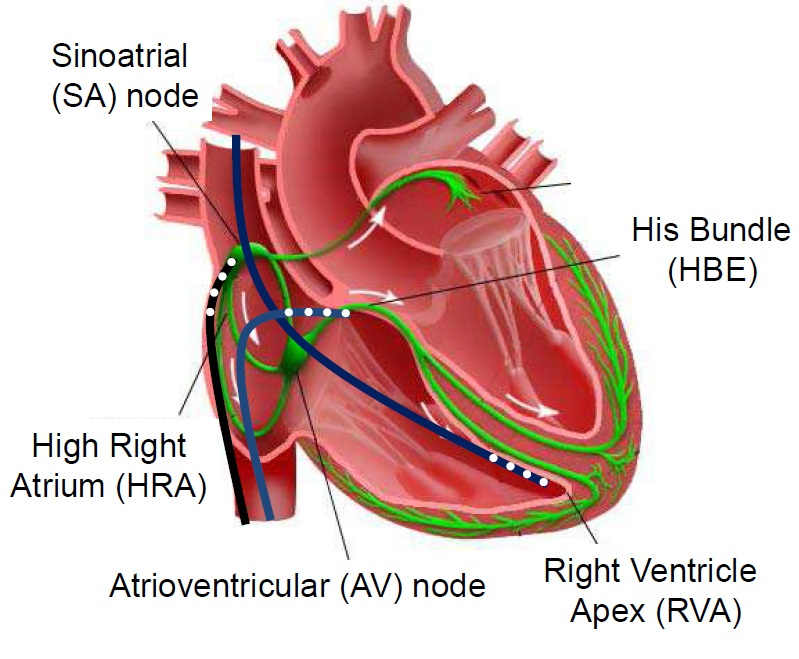
\includegraphics[width=0.262\linewidth]{figures/heart}
		} %framebox
	}
	\subfigure[The four stages of an \acf{AP}]{
		\framebox[0.31\textwidth]{
			\begin{tikzpicture}[transform shape, xscale=0.6, yscale=0.6]
\begin{axis}
[ xlabel={Time (ms)},
ylabel={Potential ({mV})},
axis y line = left,
axis x line = bottom,
xmin=0,   xmax=300,
ymin=0,   ymax=150,
ytick={0, 30, 44.5, 50, 100, 131.1, 150},
yticklabels={0, $v_R$, $v_T$, 50, 100, $v_O$, 150},
extra tick style={grid=major}
]
\addplot[color=blue!90,
mark=.,
mark size=2,
smooth,
const plot
]
table [x=t, y=v, col sep=comma] {./figures/actionPotentialData.csv};

\addplot[color=black!90,
dashed,
mark=.,
mark size=2
] coordinates {
	(0,30)
	(240,30)
};

\addplot[color=black!90,
dashed,
mark=.,
mark size=2
] coordinates {
	(0,44.5)
	(50,44.5)
};

\addplot[color=black!90,
dashed,
mark=.,
mark size=2
] coordinates {
	(0,131.1)
	(50,131.1)
};

\end{axis}

\tikzstyle{every state}=[rectangle, text centered, draw=none,text=black, draw,line width=0.3mm]

\node[state, shift={(0.2, -1.5)}, fill=green!20, inner xsep=0.0cm, minimum width=0.6cm] {RP};
\node[state, shift={(0.85, -1.5)}, fill=yellow!20, minimum width=0.5cm] {ST};
\node[state, shift={(3.00, -1.5)}, fill=red!20, minimum width=2.8cm] {ERP};
\node[state, shift={(1.50, -1.5)}, fill=blue!20, minimum width=0.5cm] {UP};
\node[state, shift={(5.15, -1.5)}, fill=green!20, minimum width=1.5cm] {RRP};
\node[state, shift={(6.40, -1.5)}, fill=green!20, minimum width=1cm] {RP};

\end{tikzpicture}
			\label{fig:actionPotential}
		}
	}
	\subfigure[An abstracted model of the conduction system]{ 
          \framebox[0.31\textwidth]{
          	\begin{tikzpicture}[->,>=stealth',semithick,scale=0.73, transform shape]

\tikzstyle{every state}=[fill=blue!20,circle,minimum size=0.1cm]

\tikzset{
	atrialCell/.style={
		fill=green!20,
		circle,
		minimum size=0.1cm,
		draw,
		line width=0.2mm
	}
}

\tikzset{
	ventricularCell/.style={
		fill=blue!20,
		circle,
		minimum size=0.1cm,
		draw,
		line width=0.2mm
	}
}

\tikzset{
	autorhythmicCell/.style={
		fill=yellow!20,
		circle,
		minimum size=0.1cm,
		draw,
		line width=0.2mm
	}
}

\draw node[atrialCell](SA) {\footnotesize SA};

\node[atrialCell](CT) [below left=0.3cm and 0.5cm of SA] {};
\node[atrialCell](CT1) [below left=0.5cm and 0cm of CT] {};

\node[atrialCell](BB) [below right=-0.1cm and 0.5cm of SA] {};
\node[atrialCell](LA) [below right=-0.1cm and 0.5cm of BB] {};
\node[atrialCell](LA1) [below right=-0.1cm and 0.5cm of LA] {};

\node[atrialCell](RA) [below left=0.4cm and -0.1cm of SA] {};
\node[atrialCell](RA1) [below left=0.5cm and 0cm of RA] {};
\node[atrialCell](CS) [below left=0.5cm and -0.3cm of RA1] {};

\node[atrialCell](OS) [below right=0.4cm and 0.2cm of SA] {};
\node[atrialCell](Fast) [below left=0.4cm and -0.1cm of OS] {};
\node[atrialCell](Fast1) [below right=0.4cm and -0.1cm of Fast] {};
\node[atrialCell](Slow) [below right=0.2cm and 0.3cm of OS] {};
\node[atrialCell](Slow1) [below right=0.4cm and -0.1cm of Slow] {};
\node[atrialCell](AV) [below right=0.2cm and 0.3cm of Fast1] {\footnotesize AV};

\node[ventricularCell](His) [right=0.3cm of AV] {};
\node[ventricularCell](His1) [below right=-0.1cm and 0.3cm of His] {};
\node[ventricularCell](His2) [below right=0.3cm and -0.1cm of His1] {};

\node[ventricularCell](RBB) [below left=0.4cm and 0.1cm of His2] {};
\node[ventricularCell](RBB1) [below right=0.4cm and -0.1cm of RBB] {};
\node[ventricularCell](RVA) [below right=0.4cm and -0.1cm of RBB1] {};

\node[ventricularCell](LBB) [below right=0.4cm and 0.2cm of His2] {};
\node[ventricularCell](LBB1) [below right=0.4cm and -0.1cm of LBB] {};
\node[ventricularCell](LVA) [below right=0.4cm and -0.1cm of LBB1] {};

\node[ventricularCell](LVS) [above right=0.3cm and 0.3cm of LVA] {};
\node[ventricularCell](LVS1) [above left=0.4cm and -0.1cm of LVS] {};
\node[ventricularCell](CSLV) [above left=0.4cm and -0.1cm of LVS1] {};

\node[ventricularCell](LV) [above right=0.1cm and 1.0cm of LVA] {};
\node[ventricularCell](LV1) [above left=1.8cm and -0.1cm of LV] {};

\node[ventricularCell](RVS) [above left=0.2cm and 0.6cm of RVA] {};
\node[ventricularCell](RVS1) [above left=0.4cm and -0.1cm of RVS] {};

\node[ventricularCell](RV) [above left=-0.1cm and 1.2cm of RVA] {};
\node[ventricularCell](RV1) [above left=0.9cm and 0.8cm of RV] {};

\path[-] (SA) edge (BB);
\path[-] (BB) edge (LA);
\path[-] (LA) edge (LA1);

\path[-] (SA) edge (CT);
\path[-] (CT) edge (CT1);

\path[-] (SA) edge (RA);
\path[-] (RA) edge (RA1);
\path[-] (RA1) edge (CS);

\path[-] (SA) edge (OS);
\path[-] (OS) edge (Fast);
\path[-] (Fast) edge (Fast1);
\path[-] (OS) edge (Slow);
\path[-] (Slow) edge (Slow1);
\path[-] (Fast1) edge (AV);
\path[-] (Slow1) edge (AV);

\path[-] (AV) edge (His);
\path[-] (His) edge (His1);
\path[-] (His1) edge (His2);
\path[-] (His2) edge (RBB);
\path[-] (RBB) edge (RBB1);
\path[-] (RBB1) edge (RVA);
\path[-] (His2) edge (LBB);
\path[-] (LBB) edge (LBB1);
\path[-] (LBB1) edge (LVA);
\path[-] (RVA) edge (LVA);

\path[-] (RVA) edge (RVS);
\path[-] (RVS) edge (RVS1);

\path[-] (RVA) edge (RV);
\path[-] (RV) edge (RV1);

\path[-] (LVA) edge (LVS);
\path[-] (LVS) edge (LVS1);
\path[-] (LVS1) edge (CSLV);

\path[-] (LVA) edge (LV);
\path[-] (LV) edge (LV1);

\end{tikzpicture}
          	\label{fig:heartNetwork} 
	  } %framebox
	}

}
  \caption{Electrical conduction systems of the heart}
  \label{fig:heartOverview}
\end{figure*}

\textbf{Contributions} of the paper are:  %{\color{red} [AVINASH. I do
%  not agree with this contribution at all, it should be removed] we
%  propose a new definition for \acf{HIOA} (see Section~\ref{sec:HA}) to
%  capture the electrical conduction system of the heart.} 
  (1) We have
developed a \emph{modular code generation} approach, for the first time
for \ac{HIOA} models (Section~\ref{sec:codeGen}), which is also semantic
preserving. The proposed approach performs code generation using a new
synchronous semantics~\cite{benveniste03} of \ac{HIOA}. More
importantly, the developed semantics is not restrictive,
unlike~\cite{alur2003generating, kim2003modular} and does not interact
with dynamic numerical solvers unlike~\cite{ptolemaeus2014system,
  bourke13zelus}. (2) We \emph{quantitatively evaluate} the efficacy of
the proposed approach relative \simulink
(Section~\ref{sec:benchmarking}) to demonstrate the scalability of the
approach relative to the best known model in published
literature~\cite{chen14}. Our experiments show that code generation is
feasible for thousands of nodes of the heart, unlike the 33-node
published model. % We have also modelled a much more realistic human heart
% as the modelled system can mimic its re-entrant behaviour.




%%% Local Variables:
%%% mode: latex
%%% TeX-master: "../DATE2016_codegen"
%%% End:
